\chapter*{Anexos} {
\section*{Secuencias de desarme utilizadas}

\begin{table}[h!]
	\centering
	\resizebox{\textwidth}{!}{%
	\begin{tabular}{|r|c|}
		\hline
		ID & Desarme \\ \hline \hline
		 $1$ & R2 D1 L3 D3 R1 B3 D2 F2 L1 R2 U3 R2 F2 D2 F1 U3 F2 D3 U3 L1 B2 L2 R2 U3 R1 U2 F2 D3 R2 U3 \\ \hline
		 $2$ & D1 F2 D3 B2 L1 B2 F2 D3 B2 L3 F2 U1 R2 B2 U3 B3 D1 R2 F3 D3 L2 R2 F2 L3 D2 U1 R2 F3 L3 B1 \\ \hline
		 $3$ & L2 U2 F1 R2 F3 R2 F3 L1 B2 R2 B1 F2 D2 U2 L2 R2 D2 B2 U3 F1 U3 L3 R2 D1 U1 B1 F3 L2 R3 F2 \\ \hline
		 $4$ & B2 F3 R1 D2 U1 L3 R2 B1 U1 F2 U2 B3 L3 B1 F1 D3 U2 R3 B3 R3 F1 R2 D1 L3 F1 L2 R3 B1 F1 U1 \\ \hline
		 $5$ & D1 R1 U2 L3 B2 R3 B3 R2 B3 L1 U1 B3 F2 L1 R1 U3 B1 U1 R2 D1 U1 B2 D2 U3 B2 U3 L2 R3 D3 F2 \\ \hline
		 $6$ & U2 L3 U3 L3 R2 U3 B2 R2 B1 U1 L3 R3 D1 R3 D2 F2 R2 B1 F3 L1 B2 D1 U1 L3 U1 R2 F3 D2 F1 R1 \\ \hline
		 $7$ & B1 F2 R3 F1 L1 B3 F2 D2 L3 R2 F3 L3 R1 D2 U1 F1 R2 F2 U3 R1 F1 D2 B2 R1 B1 R1 D3 U1 F3 R1 \\ \hline
		 $8$ & D1 U1 L1 U2 L1 R1 B1 F1 R1 D3 U3 L3 R3 D1 U2 B3 R1 U1 R1 D1 B3 F1 U2 B2 F2 D1 U1 L2 D3 F2 \\ \hline
		 $9$ & U3 R1 D3 B2 F2 U2 B3 L2 R2 F3 D2 U3 F3 L2 R1 D2 B3 D2 L2 U2 L1 U1 B1 F1 D2 L3 B2 U2 L3 U1 \\ \hline
		$10$ & L3 R1 B3 F3 U3 F2 L3 R1 D3 F3 U3 F1 D3 U3 B2 R3 B3 F3 R3 B2 F1 D2 B3 D1 B1 R1 F1 R2 U1 L2 \\ \hline
		$11$ & L3 B2 R1 B3 D1 F2 L3 B1 R1 B2 D3 B1 U1 F3 R2 D3 L2 R2 U1 B2 U2 R1 D3 U3 F1 R2 B3 F1 U2 F3 \\ \hline
		$12$ & D3 U1 L1 R1 B1 F1 R1 F2 U2 F3 L3 R2 D2 U2 F3 U3 F3 L3 B3 F1 U3 L3 B2 F1 L3 D1 L3 R2 D2 R3 \\ \hline
		$13$ & R3 D2 L1 R1 F1 L2 B1 F2 L2 D1 L2 R2 B1 F2 U2 B3 L1 U3 F1 D3 F2 L1 D1 F1 D1 F3 R1 U1 L3 F3 \\ \hline
		$14$ & B3 L2 R2 B2 F2 L1 F3 U1 F3 L3 U3 B2 F3 U2 F3 L1 D2 L3 R2 D2 F3 L2 D2 F1 D2 B3 R2 F2 D2 U1 \\ \hline
		$15$ & F1 U2 R3 U3 B1 F2 R2 D1 U1 L3 R3 B3 F1 D3 B3 F1 L3 B1 R1 U2 F3 U1 R3 D1 F3 D3 U2 L2 D2 B1 \\ \hline
		$16$ & F2 D2 L3 D3 L1 R1 D3 F3 D2 B3 U2 L1 D3 U1 L1 D3 B1 U1 R1 D3 R3 U1 R2 D3 L1 B1 R1 F3 L2 D1 \\ \hline
		$17$ & B3 F2 U1 F2 L1 R1 D1 U3 F1 U2 F2 L1 R1 D2 B1 D1 F2 R2 U3 R1 D2 U2 F3 L1 R3 F3 L3 R2 F2 L2 \\ \hline
		$18$ & B1 F3 D3 L3 B1 F2 R1 D3 L2 R1 F1 D2 F1 R3 F2 U3 B1 F2 D1 L3 U3 B2 F2 D3 L2 D3 U3 B1 U2 L1 \\ \hline
		$19$ & L3 U1 F1 D3 U3 R3 B2 U1 R2 F2 R3 B1 R1 U1 L2 B3 F3 U1 L2 R1 U3 B2 L3 U1 F1 R3 B1 L1 F2 L1 \\ \hline
		$20$ & D3 L3 R3 U2 R1 F2 L2 D3 F1 D3 R1 D2 U2 R2 F2 L2 R2 F3 R2 D3 B1 U1 B2 L1 R3 F3 D2 F1 R1 F2 \\ \hline
	\end{tabular}
	}
	\caption{Desarmes utilizados para la experimentos de visión.}
	\label{vision}
\end{table}
\newpage
\section*{Desarmes truncados}
\begin{table}[h!]
	\centering
	\resizebox{0.9\textwidth}{!}{%
	\begin{tabular}{|r|c|}
		\hline
		ID & Desarme \\ \hline \hline
		$1$ & R2 \\ \hline
		$2$ & D1 F2 \\ \hline
		$3$ & L2 U2 F1 \\ \hline
		$4$ & B2 F3 R1 D2 \\ \hline
		$5$ & D1 R1 U2 L3 B2 \\ \hline
		$6$ & U2 L3 U3 L3 R2 U3 \\ \hline
		$7$ & B1 F2 R3 F1 L1 B3 F2 \\ \hline
		$8$ & D1 U1 L1 U2 L1 R1 B1 F1 \\ \hline
		$9$ & U3 R1 D3 B2 F2 U2 B3 L2 R2 \\ \hline
	   $10$ & L3 R1 B3 F3 U3 F2 L3 R1 D3 F3 \\ \hline
	   $11$ & L3 B2 R1 B3 D1 F2 L3 B1 R1 B2 D3 \\ \hline
	   $12$ & D3 U1 L1 R1 B1 F1 R1 F2 U2 F3 L3 R2 \\ \hline
	   $13$ & R3 D2 L1 R1 F1 L2 B1 F2 L2 D1 L2 R2 B1 \\ \hline
	   $14$ & B3 L2 R2 B2 F2 L1 F3 U1 F3 L3 U3 B2 F3 U2 \\ \hline
	   $15$ & F1 U2 R3 U3 B1 F2 R2 D1 U1 L3 R3 B3 F1 D3 B3 \\ \hline
	   $16$ & F2 D2 L3 D3 L1 R1 D3 F3 D2 B3 U2 L1 D3 U1 L1 D3 \\ \hline
	   $17$ & B3 F2 U1 F2 L1 R1 D1 U3 F1 U2 F2 L1 R1 D2 B1 D1 F2 \\ \hline
	   $18$ & B1 F3 D3 L3 B1 F2 R1 D3 L2 R1 F1 D2 F1 R3 F2 U3 B1 F2 \\ \hline
	   $19$ & L3 U1 F1 D3 U3 R3 B2 U1 R2 F2 R3 B1 R1 U1 L2 B3 F3 U1 L2 \\ \hline
	   $20$ & D3 L3 R3 U2 R1 F2 L2 D3 F1 D3 R1 D2 U2 R2 F2 L2 R2 F3 R2 D3 \\ \hline
	\end{tabular}
	}
	\caption{Desarmes utilizados para la experimentos de manipulación.}
	\label{manipulation}
\end{table}

\newpage
\section*{Detalle experimentos visión}
\begin{table}[h!]
	\centering
	\resizebox{0.9\textwidth}{!}{%
		\begin{tabular}{|r|r|l|}
			\hline
			ID & Errores & Detalle \\ \hline\hline
			 $1$ & $0$ & FBBFUUFBDFRDLRUUDUDRRLFDUDFBFRLDRRFBLRLULFDBRLDUBBLLUB \\
			   &   & FBBFUUFBDFRDLRUUDUDRRLFDUDFBFRLDRRFBLRLULFDBRLDUBBLLUB \\ \hline
			 $2$ & $8$ & BFFRURRULF\underline{\textbf{U}}URR\underline{\textbf{D}}F\underline{\textbf{U}}UBF\underline{\textbf{U}}\underline{\textbf{U}}FBLURDB\underline{\textbf{D}}LDLDRBRF\underline{\textbf{U}}BLFRUBLLUBBLL\underline{\textbf{F}}F \\
			   &   & BFFRURRULF\underline{\textbf{D}}URRUF\underline{\textbf{D}}UBF\underline{\textbf{D}}\underline{\textbf{D}}FBLURDB\underline{\textbf{U}}LDLDRBRF\underline{\textbf{D}}BLFRUBLLUBBLL\underline{\textbf{U}}F \\ \hline
			 $3$ & $0$ & FDBLUBLLBDDLBRFFUUDFRDFUBULRLDRDRRRLRBBDLFUFUULDUBRFBF \\
			   &   & FDBLUBLLBDDLBRFFUUDFRDFUBULRLDRDRRRLRBBDLFUFUULDUBRFBF \\ \hline
			 $4$ & $3$ & BF\underline{\textbf{U}}U\underline{\textbf{U}}LFBRFBBDRUFDULUUUFRLUDFRRB\underline{\textbf{U}}LUFRLFUBLFBDDRRDLBRBLL \\
			   &   & BF\underline{\textbf{D}}U\underline{\textbf{D}}LFBRFBBDRUFDULUUUFRLUDFRRB\underline{\textbf{D}}LUFRLFUBLFBDDRRDLBRBLL \\ \hline
			 $5$ & $2$ & RRFDUFLUURRDFRDDBBBRFDFLFUFLFLUDLURDBF\underline{\textbf{F}}BLLRL\underline{\textbf{F}}RBDBBULDB \\
			   &   & RRFDUFLUURRDFRDDBBBRFDFLFUFLFLUDLURDBF\underline{\textbf{U}}BLLRL\underline{\textbf{U}}RBDBBULDB \\ \hline
			 $6$ & $0$ & FBBRURBLDBBRBRRFURUDLLFDUUURFLLDBRUBDFLDLFFUFDLLDBFURD \\
			   &   & FBBRURBLDBBRBRRFURUDLLFDUUURFLLDBRUBDFLDLFFUFDLLDBFURD \\ \hline
			 $7$ & $3$ & DUFUUBFDDF\underline{\textbf{F}}\underline{\textbf{F}}DRF\underline{\textbf{F}}RLUFRLFBUBRLLBLDBDRBLFRDLUBFBLRFRBLDDR \\
			   &   & DUFUUBFDDF\underline{\textbf{U}}\underline{\textbf{U}}DRF\underline{\textbf{U}}RLUFRLFBUBRLLBLDBDRBLFRDLUBFBLRFRBLDDR \\ \hline
			 $8$ & $0$ & URDDULBBLUBBFRLFURLRFFFRFUDDLRFDRUDBLFDBLUFLLRDBDBUUBR \\
			   &   & URDDULBBLUBBFRLFURLRFFFRFUDDLRFDRUDBLFDBLUFLLRDBDBUUBR \\ \hline
			 $9$ & $0$ & UFLRULUBBRBFFRFBDRLRURFURUDBBLRDLLDFRFBLLDDUDULFDBUDBF \\
			   &   & UFLRULUBBRBFFRFBDRLRURFURUDBBLRDLLDFRFBLLDDUDULFDBUDBF \\ \hline
			$10$ & $0$ & LFURUDUUDBBBFRFFDDBBLDFLFDRRRULDLDUFUBRULFBBDLUFRBRLLR \\
			   &   & LFURUDUUDBBBFRFFDDBBLDFLFDRRRULDLDUFUBRULFBBDLUFRBRLLR \\ \hline
			$11$ & $0$ & LLFUURDLLDFUDRUUFUFFBUFFFDRUBBRDUBDBFRRBLBRBRLDDLBLLRD \\
			   &   & LLFUURDLLDFUDRUUFUFFBUFFFDRUBBRDUBDBFRRBLBRBRLDDLBLLRD \\ \hline
			$12$ & $0$ & RFUBULLUBUDLDRBFDFDRLRFFDUDRLRLDRUBLFRBLLFRBBFUUDBFDUB \\
			   &   & RFUBULLUBUDLDRBFDFDRLRFFDUDRLRLDRUBLFRBLLFRBBFUUDBFDUB \\ \hline
			$13$ & $0$ & RBFRUDBDBLBUURFRFUDLDFFBLDUFRFUDLUURDBRRLDBFDLLFRBUBLL \\
			   &   & RBFRUDBDBLBUURFRFUDLDFFBLDUFRFUDLUURDBRRLDBFDLLFRBUBLL \\ \hline
			$14$ & $6$ & DFLRUDRUUBFURRBFFDFLR\underline{\textbf{U}}FB\underline{\textbf{U}}\underline{\textbf{D}}LRUDBD\underline{\textbf{L}}\underline{\textbf{B}}\underline{\textbf{F}}LFUURLLULBBRRDBDBFL \\
			   &   & DFLRUDRUUBFURRBFFDFLR\underline{\textbf{D}}FB\underline{\textbf{D}}\underline{\textbf{B}}LRUDBD\underline{\textbf{U}}\underline{\textbf{F}}\underline{\textbf{L}}LFUURLLULBBRRDBDBFL \\ \hline
			$15$ & $2$ & RLFFUUULLBRDBRRDDRFB\underline{\textbf{D}}BFRR\underline{\textbf{D}}LULBUDFFDUBRLLLULFBRFDDBDFBD \\
			   &   & RLFFUUULLBRDBRRDDRFB\underline{\textbf{U}}BFRR\underline{\textbf{U}}LULBUDFFDUBRLLLULFBRFDDBDFBD \\ \hline
			$16$ & $0$ & UBFBURBLUBDDBRDLFDUDRLFLUFBFRDFDUDUBRDLULUFLLRRFFBBRRL \\
			   &   & UBFBURBLUBDDBRDLFDUDRLFLUFBFRDFDUDUBRDLULUFLLRRFFBBRRL \\ \hline
			$17$ & $0$ & FDBUUULFRBLLBRFRDDFDDRFUUDBRBULDRBLRLRDRLFDFFULUUBBFBL \\
			   &   & FDBUUULFRBLLBRFRDDFDDRFUUDBRBULDRBLRLRDRLFDFFULUUBBFBL \\ \hline
			$18$ & $0$ & BULDUBFBLBRFFRUDLRUDUUFDDRFRDLLDFDBBLLRFLRRUBUBDFBRULF \\
			   &   & BULDUBFBLBRFFRUDLRUDUUFDDRFRDLLDFDBBLLRFLRRUBUBDFBRULF \\ \hline
			$19$ & $3$ & DULLUULUDRRURRRULUD\underline{\textbf{D}}\underline{\textbf{D}}\underline{\textbf{D}}FDFDLUFFDDBDFRFUBFLDFLRBFRBBLBRL \\
			   &   & DULLUULUDRRURRRULUD\underline{\textbf{B}}\underline{\textbf{B}}\underline{\textbf{B}}FDFDLUFFDDBDFRFUBFLDFLRBFRBBLBRL \\ \hline
			$20$ & $0$ & BRDDUUBBLBFFFRLRLFRLUBFLDDFBFDBDDUBRDRUFLULDLLURUBRURF \\
			   &   & BRDDUUBBLBFFFRLRLFRLUBFLDDFBFDBDDUBRDRUFLULDLLURUBRURF \\ \hline
		\end{tabular}
	}
	\caption[Errores visión.]{Errores visión. Esta tabla indica los facelet específicos donde el algoritmo de visión desarrollado se equivocó. En cada fila, el string superior es el resultado obtenido y el inferior el esperado. Las diferencias se muestran subrayadas y en negrita.}
	\label{visionerrors}
\end{table}

\newpage
\small{\section*{Proyecciones de colores representantes en RGB}}
\begin{figure}[h!]
	\centering
	\subcaptionbox{Proyección en ejes rojo (horizontal) y verde (vertical).}{%
	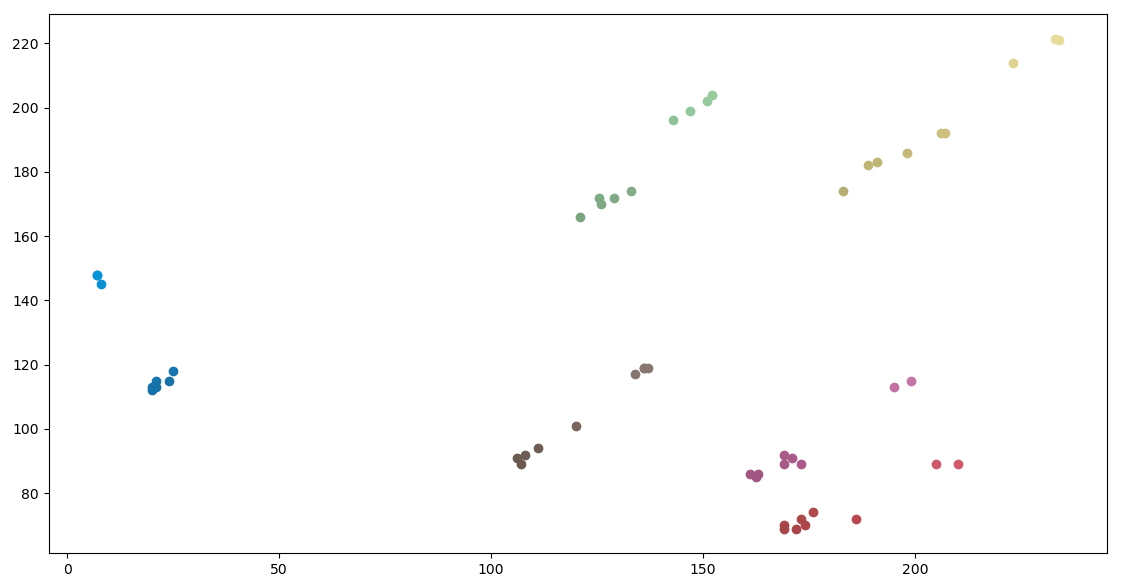
\includegraphics[width=0.65\textwidth]{figures/rg}
	}%
	\vfill
	\subcaptionbox{Proyección en ejes rojo (horizontal) y azul (vertical).}{%
	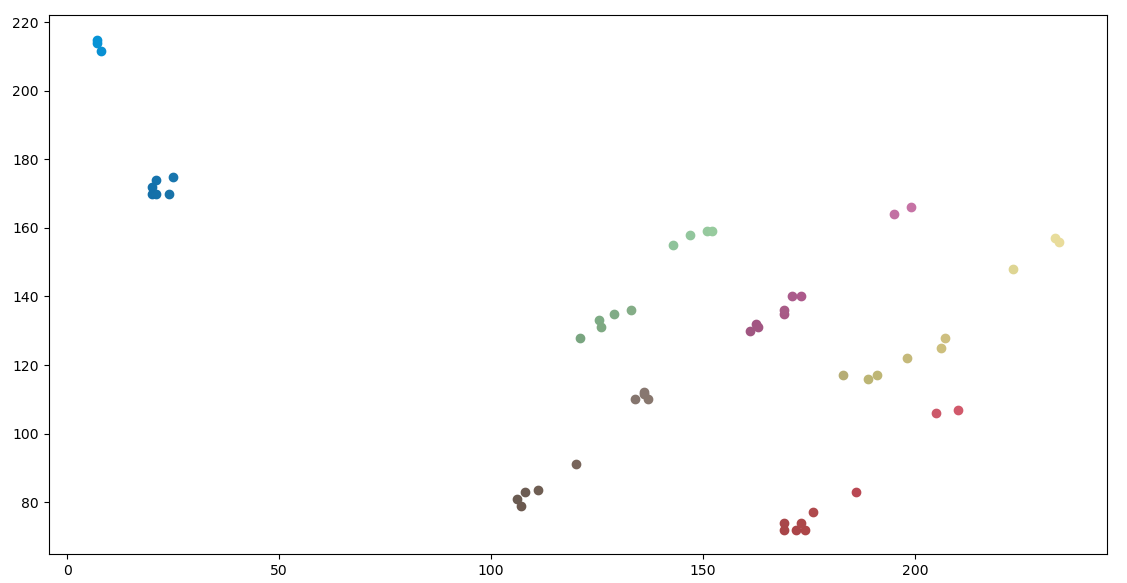
\includegraphics[width=0.65\textwidth]{figures/rb}
	}%
	\vfill
	\subcaptionbox{Proyección en ejes verde (horizontal) y azul (vertical).}{%
	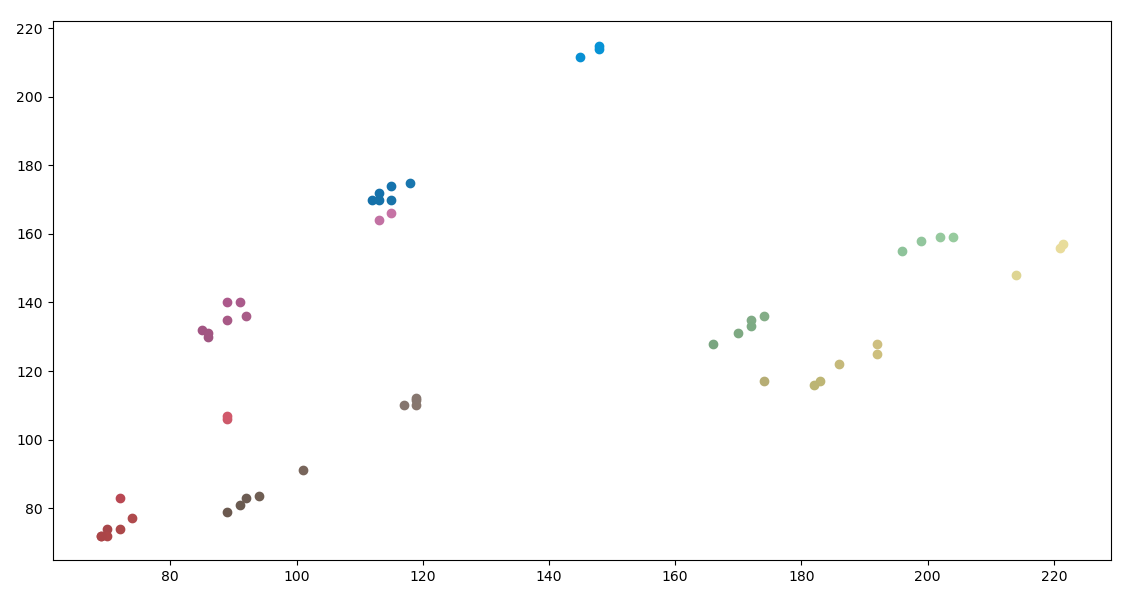
\includegraphics[width=0.65\textwidth]{figures/gb}
	}%
	\caption[Proyecciones.]{Proyecciones. Se aprecia la distribución en rectas de los facelets del mismo color.}
	\label{proyecciones}
\end{figure}

}
\newpage
\section*{Brazos del Robot}
\begin{figure}[h!]
	\centering
	\includegraphics[width=0.5\textwidth]{figures/baxter_joint_names}
	\caption{Articulaciones del robot Baxter.}
	\label{baxterjoints}
\end{figure}
\begin{figure}[h!]
	\centering
	\includegraphics[width=0.5\textwidth]{figures/baxter_arm}
	\caption{Muñeca del robot.}
	\label{baxterjoints}
\end{figure}

\newpage
\newpage
\section*{Recursos adicionales}

\begin{enumerate}
	\item Vídeo de ejemplo de Robot Baxter resolviendo el cubo. Este corresponde a la secuencia de largo 8 en los experimentos de manipulación.
	\url{https://www.youtube.com/watch?v=AlMi1rzPEQs}
	\item Repositorio de código del sistema desarrollado: \url{https://github.com/silvercobraa/memoria-de-titulo}
	\item WCA Legacy Scrambler: \url{https://www.worldcubeassociation.org/regulations/history/files/scrambles/scramble_cube.htm}
\end{enumerate}
